\textbf{Beispiel 1}\\ \\
a)\\ \\
Mit den Freiheitsgraden
\[
	\textbf{q} = \begin{bmatrix}
		\alpha , \beta , x
	\end{bmatrix}^T
\]
wird das angegebene System vollständig beschrieben.\\ \\
b)\\ \\
Freigeschnittene Körper inklusive aller wirkenden Kräfte:
\begin{figure}[h]
	\centering
	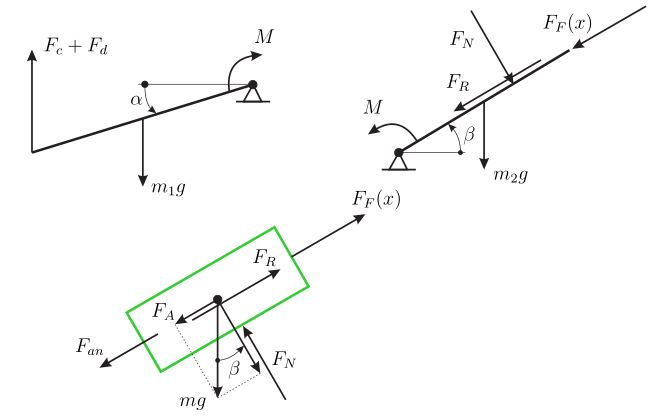
\includegraphics[width= 12cm]{tikz/23_09_2016_1b}
\end{figure}
\newline
Desweiteren gilt:
\begin{align*}
	F_c &= cl_1\sin(\alpha) \\
	F_d &= dl_1\dot{\alpha}\cos(\alpha) \\
	M &= c_D (\alpha - \beta) \\
	F_N &= mg\cos(\beta) \\
	F_A &= mg\sin(\beta)
\end{align*}
Aufgrund der Rotation des Stabes 2 wirkt auch eine Fliehkraft auf die Masse $m$. Diese lautet
\[
	F_{Flieh} = m(l_2 - x)\dot{\beta}^2
\]
c)\\ \\ 
Mit der Form der Haftreibung aus der Formelsammlung folgt die Haftbedingung
\[
	|F_{an} + F_A - F_F(x)| = |F_{an} + mg\sin(\beta) - F_F(x)| \leq mg\cos(\beta)\mu_H
\]
d)\\ \\
Die angegeben Trägheitsmomente bezieht sich jeweils auf die Schwerpunkte der Stäbe. Da sich der Drehpunkt aber am Ende der Stäbe befindet muss man hier den Satz von Steiner anwenden. 
\begin{align*}
	J_1 &= J_{S,1} + m_1\frac{l_1^2}{4} \\
	J_2 &= J_{S,2} + m_2\frac{l_2^2}{4}
\end{align*}
Durch Anwendung des Impuls- und Drallsatz folgen die Bewegungsgleichungen
\begin{align*}
	J_1\ddot{\alpha} &= m_1g\frac{l_1}{2}\cos(\beta) - c_D(\alpha - \beta) - \left(cl_1\sin(\alpha) + dl_1\dot{\alpha}\cos(\alpha)\right)l_1\cos(\alpha) \\
	J_2\ddot{\beta}&= c_D(\alpha - \beta) - m_2g\frac{l_2}{2}\cos(\beta) - mg(l_2 - x)\cos(\beta) \\
	m\ddot{x} &= F_{an} - F_F(x) - \mu_V\dot{x} + mg\sin(\beta)
\end{align*}
Diese Gleichungen können unmittelbar aus den freigeschnittenen Körpern aus Punkt b) abgelesen werden.\\ \\
e)\\ \\
Für sehr kleine Winkel können die Näherungen 
\[
	\sin(\alpha) = \alpha \, , \, \sin(\beta) = \beta
\]
verwendet werden. Daraus kann man 
\[
\cos(\alpha) = 1 \, , \, \cos(\beta) = 1
\]
schließen.\\ \\
f)\\ \\
Nein es ist nicht möglich, weil in dieser Ruhelage die Feder keine Kraft und die Drehfeder kein Moment ausübt. Dadurch können aber nicht die durch die Gewichtskräfte entstehenden Momente ausgeglichen werden können.